\chapter{Testing and Plotting}
In this chapter we want to explain how the experiments were conducted and how to interpret the plots what will be used to showcase the results of those experiments in Chapter \ref{experiments_chapter}. We also want to show how to use the testing and plotting systems implemented as part of this project.

\section{Conducting the experiments}
The process of conducting experiments encountered several challenges and fluctuations. Initially, the primary concern was to determine the appropriate number of rotations (\texttt{rots}) and distances (\texttt{dists}) for each obstacle type (explained in Table \ref{commOpt}). After experimenting with up to 30 rotations in some cases, and not getting satisfying results with seemingly any combination of other parameters, it was determined that the game's difficulty in later levels was the root of the problem, as it was impossible to play with some environments(confirmed by human players). Consequently, the game had to be adjusted and thus, there are slight variations in parameters, such as the starting speed and distances between obstacles, in the version of the ``Space-run'' game used in this thesis, as compared to the original. As per a human player's assessment, it is now possible to play all environment combinations until level 15 or even beyond. It is noteworthy that level 10 was the initial choice for the winning level, which was later shifted to level 15 to prevent the agent from settling for a mediocre policy and to find the optimal policy. However, this shift did not yield significant results, and the same behaviour could likely be achieved by increasing the number of games, allowing the $\epsilon$-greedy policy to perform random moves more frequently for an extended period. Despite this, level 15 was used in all subsequent experiments.

\begin{figure}[h]
    \centering
    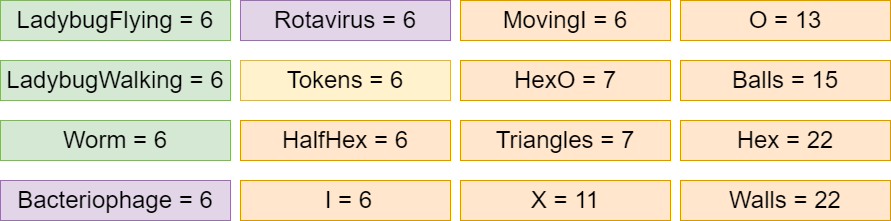
\includegraphics[width=0.8\textwidth]{rot_values}
    \caption{\texttt{rots} values used for each obstacle type}
    \label{fig:rot_values}
\end{figure}

After addressing the the issue of game not being playable, the most straightforward method for identifying the number of rotations required was to play the game manually in debug mode. The results obtained from these experiments are displayed in Figure \ref{fig:rot_values} and were used in all experiments conducted. However, for obstacles such as \texttt{Walls} and \texttt{Balls}, this method was not viable. The reason being that running \texttt{env=Balls} or \texttt{env=Walls} with visuals caused the game to lag significantly due to the number of animations playing simultaneously. As a result, \texttt{Walls} received the same number of rotations as \texttt{Hex} trap, while \texttt{Balls} received 15 rotations, the number at which the agent managed to learn. For bug, virus, and token obstacles, the default and minimum value of 6 rotations was assigned, with which they all trained successfully.
Concerning the \texttt{dists} parameter, it was concluded during the experiments that all agents could learn any obstacle with \texttt{dists=1}, and increasing this number needlessly would only increase the number of states required for training. 

The remaining values to be determined for the experiments were the suboptions for each agent (see \ref{opt:agent}).  The reader must realize that there were a lot of experiments conducted that had to be disregarded later on for this or that reason, but they provided useful insights that could be utilized. For instance, in many of those experiments, the agent performed best with \texttt{eps} values ranging from 0.2 to 0.4, with 0.2 being the most common, in combination with an \texttt{epsFinal} value of 0.0001. The rationale for using a low \texttt{epsFinal} value is that towards the end, the agent almost exclusively exploits the current policy, and a more gradual decrease in epsilon values is suitable for larger values of \texttt{n}. Furthermore, \texttt{initOptVal} of 20.0 and 100.0 was promising in most experiments. The \texttt{gam} value will be discussed in a later subsection.

Throughout the months dedicated to conducting experiments, they gradually converged towards checking combinations of the values mentioned above. In some instances, other values were experimented with and will be discussed when exploring various environments in later subsections. However, due to the length of the experiments and the number of parameters requiring adjustment, they were kept systematic towards the end, and most of the results presented in this chapter were obtained from experiments run with different \texttt{env} and value \texttt{n} adjusted according to the environment. Each combination was tested on ten seeds for each agent, with the combinations consisting of \texttt{eps} parameter taking a value of either 0.2 or 0.4, and the \texttt{initOptVal} being either 20.0 or 100.0. Discounting was kept at the value of 1 and \texttt{epsFinal} was 0.0001.

\section{Interpreting the plots}

\begin{figure}[h]
    \centering
    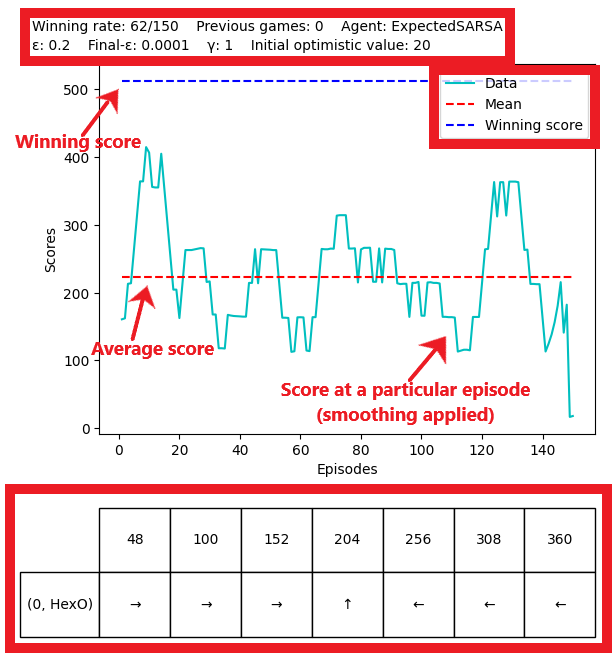
\includegraphics[width=\textwidth]{examplePlot}
    \caption{Plot example}
    \label{fig:plt_eg}
\end{figure}

In this chapter, a number of plots similar to the one shown in Figure \ref{fig:plt_eg} will be presented. This section has been dedicated to explaining the different components of these plots and how to read them. While some plots may differ slightly from the one in Figure \ref{fig:plt_eg}, the meaning behind them can still be easily deduced.

The top part of the figure displays all the necessary information that was used in the experiment. Most of the values have been previously described, except for ``Previous games''. This value is meant for experiments that used the \texttt{database=read} option and were performed on an agent that had trained for some number of games. This number specifies the how many of games the agent had previously trained on.

Moving further down, there is a plot with three lines and a legend in the top right corner. The data line, as indicated on the figure, represents the score that the agent achieved on a particular episode. However, some plots may show the average value of the agent's score for that episode over several different seeds used for the random action. Additionally, there may be multiple data lines on the plot, each averaged between many seeds and each representing a different agent. Every agent is labelled with their respective color inside the legend.

The mean line represents the average score value for the entire experiment, while the winning score represents the winning threshold which is the score that the agent achieves after passing level 15. This score will be constant, except in the cases where the environments contains any of the bugs and viruses and the agent is allowed to shoot. The winning score then depends on how many of those obstacles the agent successfully shoots. In this case the line will show the winning score of the last game in which the agent won. It should be noted that if the agent did not win any games, or the plot is displaying multiple agents, the winning score line will be omitted. Furthermore, the data line is averaged to appear smoother. This is why even though the winning rate is 62/150 in this sample plot, the data line doesn't touch the winning score threshold at any point.

As mentioned in Section \ref{commOpt}, it is possible to perform continuous evaluation on experiments, meaning one learning game is played with random actions, followed immediately by an evaluation game using only the current policy that the agent is performing. In all experiments conducted, the data line only represents the evaluation games.

At the very bottom of the figure, there is a table which only appears in plots that contain a single data line that is not averaged over different seeds and has only one seed value. In the table, all rotation values for this experiment define the columns, while each row has a tuple of distance value and type of the obstacle. Each cell then represents a particular discrete state, and the arrow it shows is the action that the agent takes in that state. If the arrow has \textit{*} attached to it, it means that the agent will also shoot. Since all experiments are performed on \texttt{dists=1}, the number of rows will match only the number of different obstacles used in the experiment.

It should be emphasized that parameters such as the number of seeds in the averaged data line or the size of the smoothing window will be clearly specified for each plot mentioned in the rest of the chapter. This prevents any form of ambiguity or confusion regarding the details of the experiment.